%%%%%%%%%%%%%%%%%%%%%%%%%%%%%%%%%%%%%%%%%%%%%%%%%%%%%%%%%%%%%%%%%%%%%%%%%%%%%%%
%
% Filename: ira-analysis.tex
% Author:   David Oniani
% Modified: August 30, 2019
%  _         _____   __  __
% | |    __ |_   _|__\ \/ /
% | |   / _` || |/ _ \\  /
% | |__| (_| || |  __//  \
% |_____\__,_||_|\___/_/\_\
%
%%%%%%%%%%%%%%%%%%%%%%%%%%%%%%%%%%%%%%%%%%%%%%%%%%%%%%%%%%%%%%%%%%%%%%%%%%%%%%%

%%%%%%%%%%%%%%%%%%%%%%%%%%%%%%%%%%%%%%%%%%%%%%%%%%%%%%%%%%%%%%%%%%%%%%%%%%%%%%%
% Document definition
%%%%%%%%%%%%%%%%%%%%%%%%%%%%%%%%%%%%%%%%%%%%%%%%%%%%%%%%%%%%%%%%%%%%%%%%%%%%%%%

\documentclass[12pt]{article}

%%%%%%%%%%%%%%%%%%%%%%%%%%%%%%%%%%%%%%%%%%%%%%%%%%%%%%%%%%%%%%%%%%%%%%%%%%%%%%%
% Packages and related settings
%%%%%%%%%%%%%%%%%%%%%%%%%%%%%%%%%%%%%%%%%%%%%%%%%%%%%%%%%%%%%%%%%%%%%%%%%%%%%%%

% Global, document-wide settings
\usepackage[margin=1in]{geometry}
\usepackage[utf8]{inputenc}
\usepackage[english]{babel}

% Bibliography and references
\usepackage[backend=biber]{biblatex}
\addbibresource{$BIB}

% Math and alignment
\usepackage{multicol}
\usepackage{bookmark}
\usepackage{adjustbox}
\usepackage{braket}
\usepackage{mathtools}
\usepackage{amsmath}
\usepackage{amssymb}
\usepackage{amsthm}
\usepackage{amsfonts}
\usepackage{algorithmic}

% Graphics
\usepackage{pgfplots}
\pgfplotsset{compat=1.16}
\usepackage{tikz}
\usetikzlibrary{cd, arrows, decorations.markings}
\usepackage{graphicx}
\usepackage{rotating}
\usepackage{pst-solides3d}
\usepackage{xcolor}

% Fancy stuff
\usepackage{fancyhdr}
\usepackage{tocloft}
\usepackage{caption}
\usepackage{soul}
\usepackage{textcomp}
\usepackage{wasysym}
\usepackage[cache=false]{minted}
\usepackage{csquotes}
\usepackage{hyperref}

%%%%%%%%%%%%%%%%%%%%%%%%%%%%%%%%%%%%%%%%%%%%%%%%%%%%%%%%%%%%%%%%%%%%%%%%%%%%%%%
% Mathematican operations and operators
%%%%%%%%%%%%%%%%%%%%%%%%%%%%%%%%%%%%%%%%%%%%%%%%%%%%%%%%%%%%%%%%%%%%%%%%%%%%%%%

% Sets and related operators
\newcommand{\nats}{\mathbb{N}}                   % Natural numbers
\newcommand{\pnats}{\mathbb{N}^+}                % Positive natural numbers

\newcommand{\ints}{\mathbb{Z}}                   % Integers
\newcommand{\pints}{\mathbb{Z}^+}                % Positive integers
\newcommand{\nints}{\mathbb{Z}^-}                % Negative integers

\newcommand{\rats}{\mathbb{Q}}                   % Rational numbers
\newcommand{\prats}{\mathbb{Q}^+}                % Positive rational numbers
\newcommand{\nrats}{\mathbb{Q}^-}                % Negative rational numbers

\newcommand{\reals}{\mathbb{R}}                  % Real numbers
\newcommand{\preals}{\mathbb{R}^+}               % Positive real numbers
\newcommand{\nreals}{\mathbb{R}^-}               % Negative real numbers

\newcommand{\irrats}{\mathbb{I}}                 % Irrational numbers

\newcommand{\pset}{\mathcal{P}}                  % Powerset
\newcommand{\card}{\abs}                         % Cardinality
\newcommand{\topology}{\mathcal{T}}              % Topology
\newcommand{\basis}{\mathcal{B}}                 % Basis
\newcommand{\oldemptyset}{\emptyset}             % Old empty set
\renewcommand{\emptyset}{\varnothing}            % New and nice empty set

% Other operators
\DeclarePairedDelimiter\abs{\lvert}{\rvert}      % Absolute value
\DeclarePairedDelimiter\ceil{\lceil}{\rceil}     % Ceiling
\DeclarePairedDelimiter\floor{\lfloor}{\rfloor}  % Floor

%%%%%%%%%%%%%%%%%%%%%%%%%%%%%%%%%%%%%%%%%%%%%%%%%%%%%%%%%%%%%%%%%%%%%%%%%%%%%%%
% Command definitions and redefinitions
%%%%%%%%%%%%%%%%%%%%%%%%%%%%%%%%%%%%%%%%%%%%%%%%%%%%%%%%%%%%%%%%%%%%%%%%%%%%%%%

% New commands
\newcommand{\rarr}{\rightarrow}                        % Leftarrow
\newcommand{\larr}{\leftarrow}                         % Rightarrow
\newcommand\und[1]{\underline{\smash{#1}}}             % Nice-looking underline

% Renewed commands
\renewcommand{\headrulewidth}{0.5pt}                   % Header rule width
\renewcommand{\footrulewidth}{0pt}                     % Footer rule width
\renewcommand{\baselinestretch}{1.5}                   % Line spacing is 1.5
\renewcommand{\cftsecleader}{\cftdotfill{\cftdotsep}}  % Dots for ToC sections

% Rename "Contents" to "Table of Contents"
\addto\captionsenglish{% Replace "english" with the language used
  \renewcommand{\contentsname}%
    {\textbf{Table of Contents}}}%

% Filling the space for centering the title of the table of contents
\renewcommand{\cfttoctitlefont}{\hspace*{\fill}\Large}
\renewcommand{\cftaftertoctitle}{\hspace*{\fill}}

%%%%%%%%%%%%%%%%%%%%%%%%%%%%%%%%%%%%%%%%%%%%%%%%%%%%%%%%%%%%%%%%%%%%%%%%%%%%%%%
% Miscellaneous
%%%%%%%%%%%%%%%%%%%%%%%%%%%%%%%%%%%%%%%%%%%%%%%%%%%%%%%%%%%%%%%%%%%%%%%%%%%%%%%

% Setting stuff
\setlength{\parindent}{0pt}  % Remove indentations from paragraphs
\frenchspacing               % Get rid of large spaces after dots
\pagestyle{fancy}            % This allows to do fancy headers and footers
\fancyhf{}                   % No additional page numbering (or other stuff)
\cfoot{\thepage}             % Display page number at the bottom, in the center

% PDF information and nice-looking urls
\hypersetup{%
  pdfauthor  = {David Oniani},
  pdftitle   = {Textual and Statistical Analysis of Russian IRA Facebook Posts},
  pdfsubject = {Statistics, Authorship Attribution, Visual Persuasion},
  colorlinks = true,
  linkcolor  = {blue!50!black},
  citecolor  = {blue!50!black},
  urlcolor   = {blue!50!black}
}

% Put a centered header of a footnote size on the top of each page
\chead{\footnotesize{\MakeUppercase{Textual and Statistical Analysis of Russian IRA Facebook Posts}}}

% Definition environment
\theoremstyle{definition}
\newtheorem*{definition}{Definition}

%%%%%%%%%%%%%%%%%%%%%%%%%%%%%%%%%%%%%%%%%%%%%%%%%%%%%%%%%%%%%%%%%%%%%%%%%%%%%%%
% Author(s), title, and date
%%%%%%%%%%%%%%%%%%%%%%%%%%%%%%%%%%%%%%%%%%%%%%%%%%%%%%%%%%%%%%%%%%%%%%%%%%%%%%%

% Author(s)
\author{David Oniani\\
        Luther College\\
        \href{mailto:oniada01@luther.edu}{oniada01@luther.edu}}

% Title
\title{\textbf{Textual and Statistical Analysis of Russian IRA Facebook Posts}\\
      {\small \textsuperscript{*}The paper is written in the scope of a
                                 collaborative summer research on visual
                                 persuasion with Richard K. Merritt.}}

% Date
\date{Month Day, Year}

%%%%%%%%%%%%%%%%%%%%%%%%%%%%%%%%%%%%%%%%%%%%%%%%%%%%%%%%%%%%%%%%%%%%%%%%%%%%%%%
% Beginning of the document
%%%%%%%%%%%%%%%%%%%%%%%%%%%%%%%%%%%%%%%%%%%%%%%%%%%%%%%%%%%%%%%%%%%%%%%%%%%%%%%

\begin{document}
\maketitle

%%%%%%%%%%%%%%%%%%%%%%%%%%%%%%%%%%%%%%%%%%%%%%%%%%%%%%%%%%%%%%%%%%%%%%%%%%%%%%%
% Abstract
%%%%%%%%%%%%%%%%%%%%%%%%%%%%%%%%%%%%%%%%%%%%%%%%%%%%%%%%%%%%%%%%%%%%%%%%%%%%%%%

\begin{abstract}
\addcontentsline{toc}{section}{Abstract}

\noindent The 2016 Presidential Election was targeted by an unprecedented
intelligence and influence campaign, arising out of Russia, it sought to
undermine the election, sow discord, attack the fissures of the United States
and sway the Election in Donald Trump’s favor. The entirety of the United
States Intelligence infrastructure acknowledge that Russians attempted to sway
the votes of millions of people. Central to this foreign infiltration into the
electorate is the merging machine learning, the principles of misdirection,
online entities deployed for the purposes of deception, and contemporary
research on persuasion, psychology and manipulation. This project not only
seeks to define the underlying dynamic design structures of this influential
campaign, but also to specifically examine how strategic design and targeted
graphic design were generated. From the contemporary political campaign to
advertisement, human actions as sociopolitical agents and consumers can be
intermediated by a contemporary influence practice. It is the contention of
this project that language and image can effectively be interengineered to
produce desired outcomes in audiences through the integrated use of specific
psychological, mnemonic and aesthetic strategies. Historically, these
strategies often use the tools of fear, racism, sexism, othering, white
supremacy and a narrowly focused patriotism. Artificial Intelligence, Content
Analysis and Machine Learning at the End of Democracy, will spend 8 weeks of
this summer using machine learning, to analyze the 3500 Russian Facebook Ad
dataset released by U.S. House of Representa- tives Permanent Select Committee
on Intelligence. We will additionally be examining the 10 million tweets and
2 million image Russian Twitter dataset. These datasets will be used as
“training data” (training data refers to refers to that portion of data used
to fit a model. Unsupervised learning refers to analysis in which one attempts
to learn something about the data. other than predicting an output value of
interest [whether it falls into clusters, for example])*. We will develop our
machine learning software in the Python computer language. We will additionally
be developing software using Google Vision artificial intelligence application
programming interface(set of tools and resources that allows software
developers to create applications) Using machine learning will allow us to
discern patterns in a very large image and text datasets. Specifically an
archive of images that were designed to manipulate the last U.S. Presidential
election. Once we discern patterns our next step is to identify images designed
to foster racism, division and the spread of intolerance.
\end{abstract}

%%%%%%%%%%%%%%%%%%%%%%%%%%%%%%%%%%%%%%%%%%%%%%%%%%%%%%%%%%%%%%%%%%%%%%%%%%%%%%%
% Table of Contents
%%%%%%%%%%%%%%%%%%%%%%%%%%%%%%%%%%%%%%%%%%%%%%%%%%%%%%%%%%%%%%%%%%%%%%%%%%%%%%%

\newpage
\tableofcontents
\newpage

%%%%%%%%%%%%%%%%%%%%%%%%%%%%%%%%%%%%%%%%%%%%%%%%%%%%%%%%%%%%%%%%%%%%%%%%%%%%%%%
% The rest of the stuff...
%%%%%%%%%%%%%%%%%%%%%%%%%%%%%%%%%%%%%%%%%%%%%%%%%%%%%%%%%%%%%%%%%%%%%%%%%%%%%%%

\section*{\centering Example Section}
\addcontentsline{toc}{section}{Example Section}

Proin~\cite{munkres2000} posuere suscipit ante, vitae eleifend nulla
rhoncus in. Etiam vitae tellus vel augue porta consectetur in et risus.
Nunc placerat in massa vel ultricies. In pharetra id odio vitae porttitor.
Donec blandit tincidunt nunc, vitae dignissim massa semper in. Nulla facilisis
imperdiet nisi dignissim suscipit. Proin auctor turpis vitae magna elementum,
vitae imperdiet nunc blandit.

\begin{figure}[H]
\centering
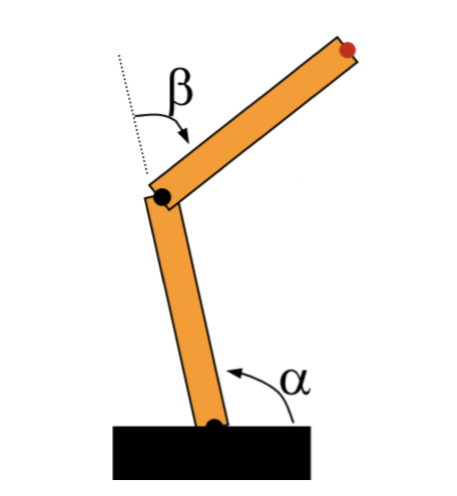
\includegraphics[width=4cm, height=4cm]{image/two-rod-system}
\caption*{A two-rod system ($2R$ robot).}
\end{figure}

Etiam arcu dui, volutpat accumsan tempor vel, blandit a quam. Sed non tortor
maximus, ullamcorper purus id, fringilla nibh. Phasellus fringilla ac massa
vel congue. Ut fringilla id quam quis condimentum. Nulla a rhoncus risus.
Morbi ut semper diam, faucibus mattis risus. Donec efficitur congue risus,
vitae varius sapien hendrerit sit amet. Duis fringilla, enim sed aliquet
gravida, dolor arcu posuere lacus, vel lacinia neque velit non sapien.

%%%%%%%%%%%%%%%%%%%%%%%%%%%%%%%%%%%%%%%%%%%%%%%%%%%%%%%%%%%%%%%%%%%%%%%%%%%%%%%
% Bibliography and references
%%%%%%%%%%%%%%%%%%%%%%%%%%%%%%%%%%%%%%%%%%%%%%%%%%%%%%%%%%%%%%%%%%%%%%%%%%%%%%%

\newpage

\begin{center}
\printbibliography[heading=bibintoc]
\end{center}

%%%%%%%%%%%%%%%%%%%%%%%%%%%%%%%%%%%%%%%%%%%%%%%%%%%%%%%%%%%%%%%%%%%%%%%%%%%%%%%
% The end of the document
%%%%%%%%%%%%%%%%%%%%%%%%%%%%%%%%%%%%%%%%%%%%%%%%%%%%%%%%%%%%%%%%%%%%%%%%%%%%%%%

\end{document}
